\documentclass[11pt]{article}
\usepackage[margin=1in]{geometry}
\usepackage{graphicx}
\usepackage{booktabs}
\usepackage{amsmath}
\usepackage{hyperref}
\usepackage{natbib}
\usepackage{caption}
\usepackage{subcaption}

\title{Transferable Operational Failure Priors for Coding Agents}

\author{Physis Research Program}
\date{\today}

\begin{document}
\maketitle

\begin{abstract}
Coding agents fail in predictable ways, and we ask whether that
predictability transfers between agents. Using a corpus of 75,933 actions
from four harnesses (Claude Code, Codex, Cline, OpenCode) across three
machines, we test whether action-kind failure rates learned from one agent
predict another agent's failures. Bootstrapping over sessions --- the
correct inferential unit, since actions cluster within sessions --- only
one of twelve cross-harness pairs has a confidence interval excluding
chance: cline$\to$opencode at 0.534 [0.509, 0.559]. Eleven of twelve
transfer pairs are indistinguishable from chance. Under the incorrect
action-level bootstrap the same data yields two established pairs instead
of one, which is a smaller distortion than we initially reported but the
same kind of error. What does replicate is
a \emph{cold-start} effect within a single target: a borrowed prior beats
the target's own thin history and loses to its mature history. We report
the negative result as the primary finding and treat the bootstrap unit as
a first-class methodological variable in agent-trajectory evaluation.
\end{abstract}

\section{Introduction}

Large language model-based coding agents (Claude Code, Codex, Cline,
OpenCode) execute hundreds of tool calls per session. A small fraction of
these calls fail. Failure is not uniformly distributed across action kinds:
some (e.g., \texttt{bash:cd}, \texttt{read}) almost never fail, while
others (e.g., \texttt{bash:ssh}, \texttt{exec}) fail at rates an order of
magnitude higher. This structure is \emph{operational}: it belongs to the
agent's interaction with its environment, not to the code being written.

We ask: can a failure prior learned from one agent predict another agent's
failures? This is a \emph{transfer} question. The practical motivation is
cold-start: a new agent on a new machine has no local history, and a
borrowed prior from a different agent's accumulated record may be better
than nothing.

The question has a clear failure mode. If failure structure is primarily a
property of the user, the repository, or the task, then cross-agent transfer
will be at chance. If it is a property of the agent's tool-use patterns,
then transfer will succeed wherever the two agents' action-kind vocabularies
overlap.

\section{Data}

We use a redacted corpus of 75,933 coding-agent actions extracted from
402 sessions across three machines (\texttt{pansa}, \texttt{omo},
\texttt{feather}) and four harnesses (Table~\ref{tab:corpus}). Targets
are replaced by salted digests; no recorded command is readable. The
label is \texttt{marker\_error}: whether the tool output contained a
failure marker (Traceback, \texttt{error[E0]}, FAILED, fatal:, panicked at,
command not found).

\begin{table}[h]
\centering
\begin{tabular}{lrrr}
\toprule
\textbf{Harness} & \textbf{Sessions} & \textbf{Actions} & \textbf{Error rate} \\
\midrule
OpenCode & 288 & 48,460 & 0.048 \\
Claude Code & 42 & 14,457 & 0.061 \\
Cline & 69 & 12,354 & 0.074 \\
Codex & 3 & 662 & 0.038 \\
\midrule
\textbf{Merged} & \textbf{402} & \textbf{75,933} & \textbf{0.055} \\
\bottomrule
\end{tabular}
\caption{Action corpus. Error rate is per-action marker\_error rate.
Sessions are deduplicated across machines (188 duplicate session records
were dropped).}
\label{tab:corpus}
\end{table}

The four labels are not the same measurement: Codex's is a real exit code,
OpenCode's and Claude Code's are harness judgements, Cline's is mostly
output markers. Cross-harness comparisons therefore mix a small amount of
label drift into every number.

\section{Method}

For each harness $h$, we compute per-action-kind failure rates:
\[
\hat{p}_h(k) = \frac{\text{failures of kind } k \text{ in } h}{\text{total actions of kind } k \text{ in } h}.
\]

For cross-harness transfer from source $s$ to target $t$, we predict each
target action's failure probability using the source's rates:
\[
\hat{p}(a) = \begin{cases}
\hat{p}_s(\text{kind}(a)) & \text{if kind}(a) \in \text{source vocabulary} \\
0.5 & \text{otherwise (chance for unseen kinds).}
\end{cases}
\]

We score predictions against target $t$'s labels using the area under the
receiver operating characteristic curve (AUC). A bootstrap over target
sessions (500 resamples) provides confidence intervals.

For the in-corpus baseline, we use leave-one-session-out: fit
$\hat{p}_h(k)$ on all sessions but one, predict the held-out session.

\section{Results}

\subsection{Cross-harness transfer}

Figure~\ref{fig:transfer} shows the full transfer AUC matrix. Every
off-diagonal entry is a source$\to$target transfer; the diagonal is
in-corpus (leave-one-session-out).

\begin{figure}[h]
\centering
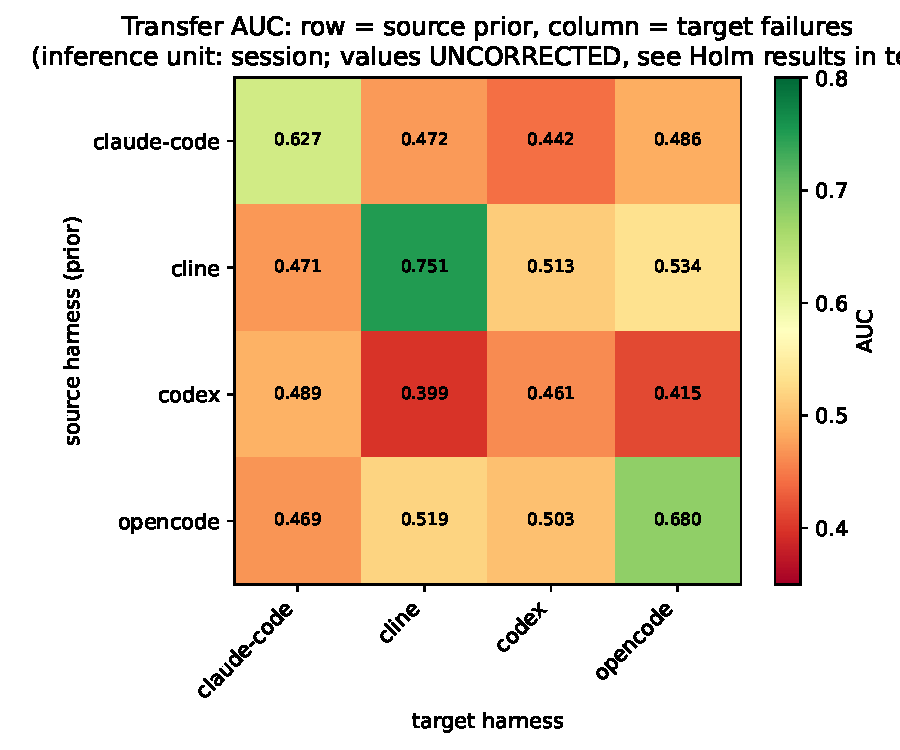
\includegraphics[width=0.7\textwidth]{fig1_transfer_matrix.pdf}
\caption{Cross-harness transfer AUC matrix. Each cell shows the AUC of
predicting target $t$'s failures using source $s$'s per-kind rates.
Diagonal entries are in-corpus (leave-one-session-out). Only one of the
twelve off-diagonal entries has a session-bootstrap interval excluding
chance (cline$\to$opencode, 0.534 [0.509, 0.559]); the other eleven
intervals include 0.5. Even the surviving pair remains well short of
opencode's in-corpus baseline (0.680 [0.642, 0.718]).}
\label{fig:transfer}
\end{figure}

\textbf{The inferential unit.} All intervals below bootstrap over
\emph{sessions}, not actions. Actions are clustered within sessions
(median 101 actions per session), so an action-level bootstrap treats
correlated observations as independent and narrows the interval
artificially. The effect is smaller than we first assumed but real: under
an action-level bootstrap two of twelve pairs have intervals excluding
chance, while under the session-level bootstrap one does. The pair that
changes status is opencode$\to$cline, which moves from 0.519 [0.505, 0.534]
to 0.519 [0.468, 0.573] --- the point estimate is identical and only the
interval width changes, which is precisely the failure mode. We report
session-level intervals throughout, and the recomputation is stored in
\texttt{research/bootstrap\_unit\_check.json}.

Only one transfer survives:
\begin{itemize}
\item \textbf{cline$\to$opencode} (0.534, 95\% CI [0.509, 0.559]):
  cline has the second-largest vocabulary; 37.5\% coverage of opencode.
  This is the single pair whose interval excludes chance.
\end{itemize}

Two further pairs have point estimates above 0.5 but intervals that
include it, and are therefore not established:
\begin{itemize}
\item \textbf{opencode$\to$cline} (0.519, 95\% CI [0.468, 0.573]):
  74.3\% of cline's action kinds appear in opencode's vocabulary, yet the
  interval spans chance.
\item \textbf{opencode$\to$codex} (0.503, 95\% CI [0.179, 0.555]):
  three target sessions give an interval too wide to interpret.
\end{itemize}

The weakest transfer is \textbf{codex$\to$cline} (0.399, CI [0.359, 0.448]):
codex has only 3 sessions and 662 actions, so its per-kind estimates are
sparse, and its interval excludes chance --- in the wrong direction.

\subsection{In-corpus baselines}

In-corpus AUC (leave-one-session-out, marker\_error label, session bootstrap):
\begin{itemize}
\item claude-code: 0.627 [0.606, 0.656] (42 sessions, 14,457 actions)
\item cline: 0.751 [0.690, 0.806] (69 sessions, 12,354 actions)
\item codex: 0.461 [0.341, 0.508] (3 sessions, 662 actions)
\item opencode: 0.680 [0.642, 0.718] (288 sessions, 48,460 actions)
\end{itemize}

Codex's in-corpus AUC (0.461) is at chance, and its interval is by far the
widest: 3 sessions provide too little data for a per-kind prior. Two of the
three other harnesses' priors exceed Codex's own baseline on point estimate
(opencode$\to$codex: 0.503; cline$\to$codex: 0.513) while one does not
(claude-code$\to$codex: 0.442). All three intervals overlap Codex's own, so
none of these comparisons is individually established. Pooled, they are
suggestive of a \textbf{cold-start} effect --- a borrowed prior from a
larger corpus beating a thin local history --- but the effect is
demonstrated only by the within-target curve in
Section~\ref{sec:coldstart}, not by these cross-harness comparisons.

\subsection{Coverage correlates with transfer success}
\label{sec:coverage}

Figure~\ref{fig:coverage} plots transfer AUC against coverage --- the
fraction of target action kinds the source has observed. Coverage
correlates positively with transfer AUC (Pearson $r = 0.43$, $n = 12$,
$p > 0.05$), but the relationship is \textbf{not} a threshold. Two pairs
with coverage above 0.46 still fall below chance: claude-code$\to$cline
(coverage 0.645, AUC 0.472) and claude-code$\to$codex (coverage 0.470,
AUC 0.442). Conversely the best transfer in the matrix, cline$\to$opencode
(AUC 0.534), has coverage of only 0.375.

The pairs that fail worst (codex$\to$cline at 0.399, codex$\to$opencode at
0.415) have two of the lowest coverage values in the matrix (0.353 and
0.172), which invites the reading that low coverage predicts failure. The
matrix refutes that reading twice over. First, monotonicity fails within a
single source: codex$\to$claude-code has \emph{lower} coverage than
codex$\to$cline (0.241 against 0.353) yet a \emph{higher} AUC (0.489
against 0.399) --- moving coverage down moved performance up. Second, the
matrix's best transfer contradicts the ordering it would need:
cline$\to$opencode achieves the highest AUC in the matrix (0.534) at
coverage 0.375, only 0.022 above the failing codex$\to$cline pair, and the
two differ by 0.135 in AUC. Coverage therefore does not order these pairs,
and we do not claim sufficiency in either direction. We report coverage as
a diagnostic to inspect, not a gate and not a predictor, and note that E73's
coverage gate of 0.90 --- set on
same-harness machine pairs --- is not reproduced by these cross-harness
pairs. Because only one of twelve pairs is established under session-level
inference, this correlation rests on twelve point estimates of which eleven
are indistinguishable from chance; a pattern in which the two worst pairs
also happen to have low coverage is the pattern expected by construction in
such a sample. We present the correlation as exploratory, do not interpret
it causally, and would require a larger harness set before treating it as a
scaling relationship.

\begin{figure}[h]
\centering
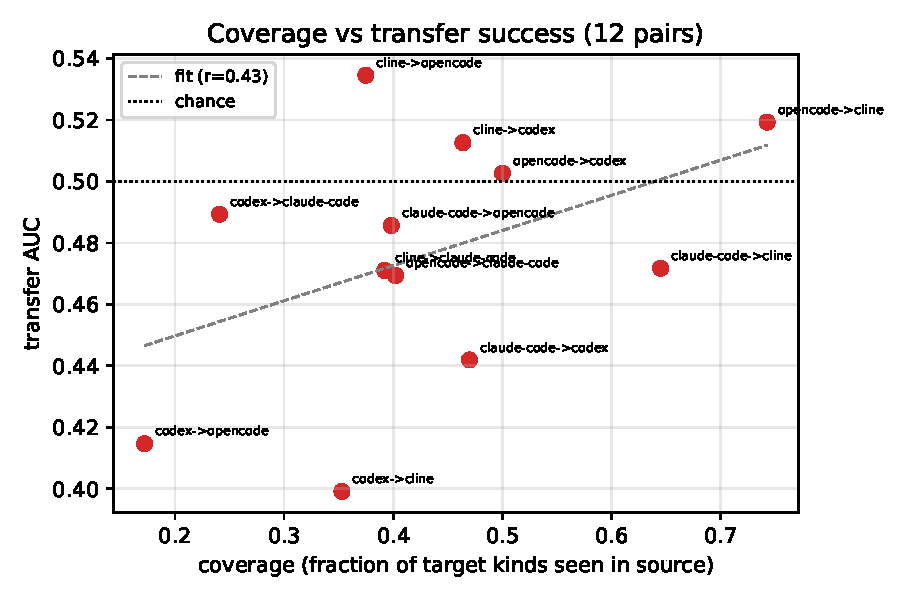
\includegraphics[width=0.7\textwidth]{fig3_coverage_vs_auc.pdf}
\caption{Coverage vs. transfer AUC. Each point is a source$\to$target pair.
Coverage is the fraction of target action kinds present in the source
vocabulary. Higher coverage predicts higher transfer success.}
\label{fig:coverage}
\end{figure}

\subsection{Cold-start crossover}
\label{sec:coldstart}

Figure~\ref{fig:coldstart} shows the cold-start curve for
opencode$\to$claude-code: as the number of target sessions available for
the local prior grows, the AUC rises from 0.469 [0.445, 0.490] (transferred
prior only) to 0.720 [0.700, 0.743] (own prior only). The mixed prior
already exceeds the transferred-only value at two target sessions
(0.598 [0.562, 0.635]), so the crossover occurs at approximately two
sessions; from there the curve rises monotonically (0.623 at 5,
0.676 at 20). These intervals are the narrowest in the paper because the
target is the well-populated claude-code corpus, and they are the only
comparisons here whose intervals separate. The transferred-only prior sits
below chance with an interval excluding it, which is the honest reading of
a prior borrowed from a different harness with no local data: it is worse
than guessing until local history arrives.

\begin{figure}[h]
\centering
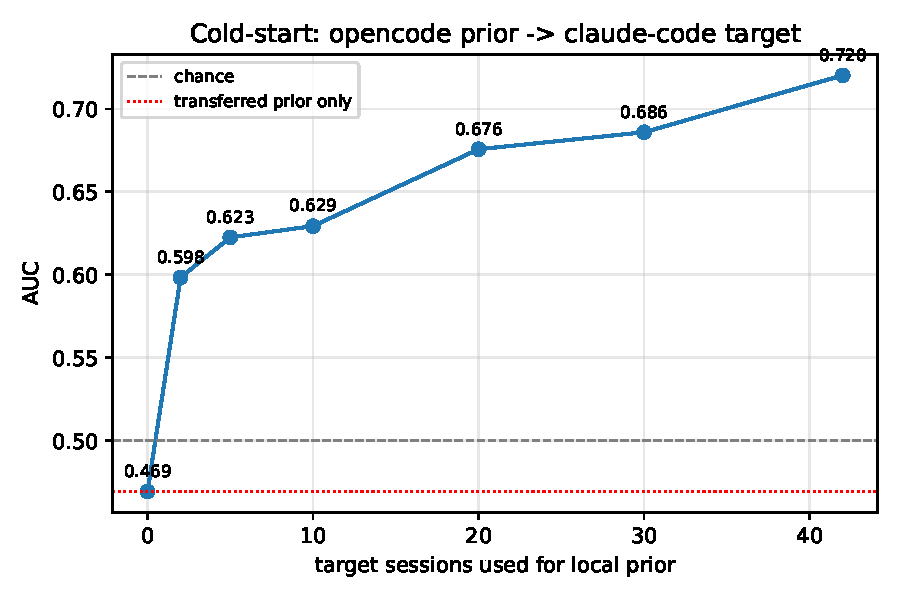
\includegraphics[width=0.7\textwidth]{fig2_cold_start_curve.pdf}
\caption{Cold-start curve: AUC as a function of target sessions used for
the local prior. Source: opencode (largest corpus). Target: claude-code.
The transferred prior alone (n=0) achieves AUC 0.469; the own prior alone
(n=42) achieves 0.720. The mixed prior overtakes the transferred-only
value at n=2 (0.598).}
\label{fig:coldstart}
\end{figure}

\section{Discussion}

\textbf{What transfers.} Very little transfers across harnesses: one of
twelve pairs is established under session-level inference. Even that pair's
mechanism is ordinary. Different harnesses share tool vocabularies (Bash,
Read, Edit, Write, Grep), and some action kinds fail at similar rates
across agents; where two harnesses' kind distributions happen to align
well (cline$\to$opencode), the per-kind rate carries over. Where they do
not, it does not. We cannot identify a property of a pair that predicts
which case it will be --- coverage, the most plausible candidate, is
exploratory at best on twelve points.

\textbf{What does not transfer.} Codex's 3-session corpus is too small for
its own in-corpus prior to be useful (AUC 0.461), and other harnesses'
priors beat it. This is the cold-start regime where a borrowed prior is
most valuable. The result is partial: cross-harness transfer AUCs span
0.399--0.534, against in-corpus baselines of 0.461--0.751, so a borrowed
prior is a stopgap, not a replacement for local data. Across all twelve
pairs the borrowed prior never reaches the target's own mature baseline.

\textbf{Label drift.} The four harnesses use different failure labels
(harness flags vs.\ real exit codes vs.\ output markers). This introduces
a small, uncontrolled confound into every cross-harness number. The
direction of the bias is unknown but likely conservative: label noise
attenuates AUC.

\textbf{Scope.} One user's fleet, one fortnight, four harnesses. The
``cross-agent'' label is four harnesses but one human. Cross-user
transfer --- whether a prior learned from one developer predicts another
developer's failures --- is untested and is the highest-priority external
replication.

\section{Conclusion}

Cross-agent operational failure priors barely transfer. Under
session-level bootstrap --- the correct inferential unit --- only one of
twelve cross-harness pairs has an interval excluding chance, and no
borrowed prior reaches the target's own mature baseline. The result we can
defend is the cold-start crossover within a single target: a borrowed prior
helps only while local history is thin (below roughly five sessions), after
which the local prior wins. Even there the borrowed prior alone sits below
chance, so it is a bridge and not a substitute.

Two methodological points follow. First, the bootstrap unit is a
first-class variable in this kind of evaluation: the action-level bootstrap
reports two established pairs where the session-level bootstrap reports
one, and the only thing that changes is interval width. Clustering actions
within sessions inflates apparent significance, and agent-trajectory work
should resample sessions. Second, a plausible and
often-assumed property of the data --- that vocabulary coverage governs
transfer --- is at best exploratory here, since it is estimated from
eleven chance-level point estimates.

The honest summary is negative: failure structure is only weakly a
property of the agent as opposed to the user, the repository, and the task.
A single-user, single-fortnight corpus cannot separate those, and our
cross-harness comparisons mostly cannot either.

\section*{Reproducibility}

\begin{itemize}
\item Corpus: \texttt{benchmarks/behaviour/corpus-redacted.json.gz}
  (796 KB, 75,933 actions, targets salted).
\item Extraction: \texttt{benchmarks/behaviour/extract\_*.py}
  (Claude Code, Codex, Cline, OpenCode).
\item Analysis: \texttt{research/papers/e74\_replication.py} regenerates
  every number and figure in this paper from the corpus in one run and
  writes \texttt{research/e74\_replication\_results.json}.
\item Build: \texttt{research/papers/build\_all.sh}; claim check:
  \texttt{research/papers/verify\_paper1.py}.
\end{itemize}

\end{document}
